\section[Režimy a provoz neutronových detektorů]{Základní dělení, charakteristiky, provozní režimy a konfigurace provozních parametrů detektorů neutronů}

\subsection{Princip detekce neutronů}

Neutron je elektricky neutrální, proto pokud ho chceme detekovat, musíme postupovat nepřímo. Je potřeba neutron konvertovat na jinou nabitou částici (elektron, alfa, proton, ...), která se potom snáze detekuje. 

Detekce prostřednictvím sekundárních částic. Používají se detektory nabitých částic s konverzním materiálem naneseným na povrchu detektoru, někdy je konvertor přímo v aktivní části detektoru jako plyn, aby vznikající sekundární ionizující záření mohlo být bezprostředně detekováno. 

\subsubsection{Konvertor neutronů}

Konvertory neutronů představují klíčovou součást detektorů určených k měření neutronového záření. Jejich návrh a konstrukce musí splňovat následující požadavky.

\textbf{Požadavky na konvertor neutronů:}

\begin{itemize}
    \item \textbf{Velký účinný průřez:} Materiál použitý v konvertoru musí mít co největší účinný průřez pro jadernou reakci, při níž dochází ke konverzi neutronu.
    \item  \textbf{Dostupnost materiálu:} Nuklid použitý jako terč by měl být dostatečně zastoupen v přírodním izotopickém složení, nebo musí existovat cenově efektivní a účinný způsob získávání obohaceného materiálu.
    \item  \textbf{Energie uvolněná při reakci (Q-hodnota):} Energie uvolněná při konverzní jaderné reakci (Q) je důležitým parametrem. Vyšší hodnota Q umožňuje snazší potlačení doprovodného gama záření.
\end{itemize}

\textbf{Požadavky na konstrukci detektoru:}

Detektor musí být navržen tak, aby částice vzniklé při konverzní reakci odevzdaly celou svou kinetickou energii v jeho aktivním objemu. Aktivní délka detektoru musí být proto dostatečná, aby zajistila kompletní absorpci energie.

\textbf{Typy konvertorů podle skupenství:}

\begin{itemize}
    \item  \textbf{Plynné konvertory:} Ionizační a proporcionální plynové komory využívající plynný konvertor ($^3$He, $^{10}$BF$_3$).
    \item  \textbf{Kapalné konvertory:} Kapalné scintilátory.
    \item \textbf{Pevné konvertory:} 
    \begin{itemize}
        \item  Plynové komory s pevným konvertorem (např. s vrstvou $^{10}\text{B}$, $^{235}$U).
        \item  Scintilátory ($^6$LiI(Eu)).
        \item  Polovodičové detektory (konvertor nanesený nad PN přechodem).
        \item  Termoluminiscenční detektory (z $^6$LiF, dochází k excitaci elektronů, které zamrznou v mřížce. Po následném ohřátí se uvolní a změří).
        \item  Plastové nebo emulzní detektory zaznamenávající stopy neutronů.
    \end{itemize}
\end{itemize}

Citlivost detektoru závisí na hustotě atomů v konvertoru (počet atomů na $\text{cm}^3$). Vyšší hustota atomů zvyšuje citlivost na neutrony, avšak zároveň i na gama záření. Proto nelze jednoznačně preferovat konkrétní skupenství materiálu konvertoru; volba závisí na specifických požadavcích konkrétní aplikace.

Většina detektorů má on-line odezvu, ale existují i detektory, které se musí později vyhodnotit (TLD, aktivační fólie). Účel měření neutronů může být:

\begin{itemize}
    \item fluence neutronů (neutronový tok),
    \item spektrometrie neutronů (mimo počtu částic zaznamenáváme i jejich energie),
    \item měření ekvivalentní dávky (dozimetry).
\end{itemize}
  
Nejčastější reakce pro konverzi neutronu na nabitou částici jsou:

\[
^3\text{He} + ^1\text{n} \to ^3\text{H} + ^1\text{p} + 0{,}765 \, \text{MeV} \ \ \text{(He detektor)}
\]
\[
^{10}\text{B} + ^1\text{n} \to ^7\text{Li} + \alpha + 2{,}3 \, \text{MeV} \ \ \text{(B detektor, scintilátor)}
\]
\[
^{10}\text{B} + ^1\text{n} \to ^7\text{Li} + \alpha + 2{,}8 \, \text{MeV} \ \ \text{(B detektor, scintilátor)}
\]
\[
^6\text{Li} + ^1\text{n} \to ^3\text{H} + \alpha + 4{,}79 \, \text{MeV}  \ \ \text{(Scintilátor)}
\]
\[
^{235}\text{U} + ^1\text{n} \to \text{FP} + 195 \, \text{MeV}  \ \ \text{(štěpné komory)}
\]

%Pro detekci sekundárních nabitých částic se používají plynové, scintilační, polovodičové a další detektory. Konvertorem je helium a bór v plynné fázi, resp. bór a lithium (Li) v pevné fázi. Největší problém detektorů neutronů je "odfiltrování" doprovodných jevů (zejména doprovodného $\gamma$).


Základem nastavení jak plynových, tak scintilačních detektorů je kombinace vysokého napětí (zesílení ve fotonásobiči) a zesílení (v zesilovači), tak aby výsledné pulsy měly amplitudu vhodnou pro další zpracování. Dále je nutno nastavit diskriminaci, tak aby optimálně splňovala následující kombinaci požadavků:

\begin{itemize}
    \item Malá změna (nestabilita) vysokého napětí by měla mít za následek minimální změnu četnosti pulsů. Tzn. nastavení v oblasti lokálního minima nebo aspoň ploché části amplitudového spektra.
    \item Pulsy iniciované neutrony by měly být minimálně potlačeny (nesnižovat citlivost).
    \item Maximálně by měly být potlačeny pulsy iniciované $\gamma$ zářením.
\end{itemize}

Diskriminace se stanovuje z amplitudového spektra, které je spolu s voltampérovou charakteristikou základními charakteristikami detekčního řetězce.

Důležitým parametrem detektoru je citlivost; ta určuje jeho použitelnost v praxi. Citlivostí detektoru rozumíme podíl četností na konci detekčního řetězce a toku neutronů. Citlivost záleží na spektru neutronů a k její stanovení je potřeba stanovit absolutní hustotu toku, tak spektrum neutronů. 

\subsection{Základní dělení}
Tohle jsou tak nějak všechny možné detektory neutronů, co jsem byl schopen najít:
\begin{itemize}
    \item Plynové detektory
    \item Scintilátory
    \item Polovodičové detektory
%    \item Diamantové detektory
    \item Samonapájecí detektory (SPD)
    \item Termoluminiscenční detektory (TLD)
    \item Aktivační detektory
%    \item Detektory stop v pevné fázi
\end{itemize}

\subsubsection{Plynem plněné detektory}

Plynem plněné detektory patří k nejrozšířenějším detektorům ionizujícího záření. Měří ionizaci produkovanou průchodem nabité částice prostředím. Jsou založeny na sběru iontů a elektronů vytvořených dopadajícím zářením v prostoru detektoru. Ionizace je způsobena buď přímo ionizujícím zářením ($\alpha$, $\beta$), nebo interakcí nepřímo ionizujícího záření (elektromagnetické, neutrony) s materiálem detektoru.

Plynové detektory měřící neutrony mají stejné uspořádání jako pro nabité částice. 
Konvertor je nuklid s vysokým účinným průřezem pro neutrony (nejčastěji $^1$H, $^3$He, $^6$Li, $^{10}$B, $^{235}$U). Nejčastěji je obsažen v plynové náplni nebo materiálu pokrývajícím stěny detektoru. Plynové detektory pracují nejčastěji v režimu ionizační komory nebo proporcionality.

Plynné prostředí plynové detektoru je řídké, což je výhoda z hlediska nízké citlivost ke $\gamma$ záření, ale na druhou stranu celková nižší účinnost kvůli menšímu účinnému průřezu.

\textbf{Borové komory:}

Borové komory využívají reakci $^{10}\text{B}(n, \alpha)$. Bór může být buď nanesený na vnitřní straně stěny komory, nebo použit jako plynová náplň BF$_3$. 

Reakce probíhají dle následujících rovnic:
\[
^{10}_5\text{B} + ^1_0\text{n} \rightarrow ^7_3\text{Li} + ^4_2\alpha \quad Q = 2{,}790\,\text{MeV} \quad (6\%)
\]
\[
^{10}_5\text{B} + ^1_0\text{n} \rightarrow ^7_3\text{Li}^* + ^4_2\alpha + \gamma(0{,}48\,\text{MeV}) \quad Q = 2{,}310\,\text{MeV} \quad (94\%)
\]

Příklady borových komor: SNM10, SNM12, používané například na reaktoru VR-1.

\textbf{Lithiové, heliové a gadoliniové komory}

Lithiové komory využívají reakci $^6\text{Li}(n, \alpha)$:
\[
^6_3\text{Li} + ^1_0\text{n} \rightarrow ^3_1\text{H} + ^4_2\alpha \quad Q = 4{,}784\,\text{MeV}
\]

Heliové komory pracují na základě reakce $^3\text{He}(n, p)$:
\[
^3_2\text{He} + ^1_0\text{n} \rightarrow ^3_1\text{H} + ^1_1\text{p} \quad Q = 0{,}764\,\text{MeV}
\]

Gadoliniové komory využívají reakce $^{157}\text{Gd}(n, \gamma)$ a vyznačují se velmi vysokou citlivostí. Pro jejich správnou funkci je nutná diskriminace gama záření.

\textbf{Štěpné komory:}

Štěpné komory pracují na základě štěpných reakcí s izotopy $^{235}\text{U}$, $^{233}\text{U}$ a $^{239}\text{Pu}$:
\[
^{235}\text{U}, ^{233}\text{U}, ^{239}\text{Pu} (n, f)
\]

Na povrchu štěpné komory je štěpný materiál, jako je $^{235}\text{U}$, $^{233}\text{U}$ nebo $^{239}\text{Pu}$, což je vhodné pro detekci tepelných neutronů. Štěpitelné materiály jako $^{238}\text{U}$ a $^{232}\text{Th}$ se používají pro detekci rychlých neutronů.

Je nutné diskriminovat vliv $\alpha$ záření ze štěpných nebo štěpitelných materiálů. Štěpné komory jsou citlivé také na gama záření, což vyžaduje další diskriminaci.

Příklad použití: Štěpné komory RJ1300 na reaktoru VR-1. Tyto komory zahrnují i miniaturizované varianty s průměrem jen 4,7 mm, které jsou vhodné pro vnitro-reaktorová měření (in-core měření).

\textbf{Klasifikace plynových detektorů}

\begin{figure}[H] 
    \centering
    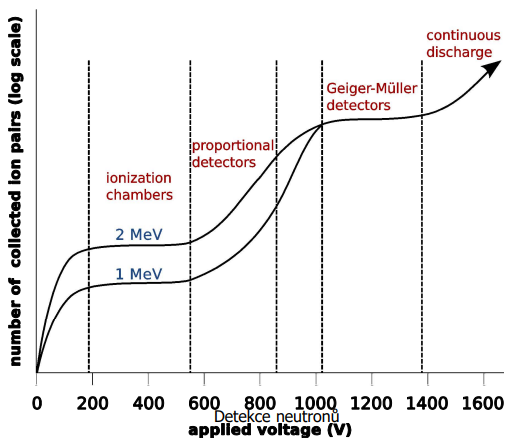
\includegraphics[width=0.5\textwidth]{img/KlasifikacePlynovýchDetektorů.png}
    \caption{Klasifikace plynových detektorů.}
    \label{fig:KlasifikacePlynovýchDetektorů}
\end{figure}

Klasifikace plynových detektorů zahrnuje několik typů, z nichž každý má své specifické vlastnosti a použití.

Ionizační komory pracují tak, že volba napětí zajistí, aby proud komorou nezávisel na napětí (nasycený proud). Odezva komory závisí i na energii záření a může být provozována impulzně i proudově.

Proporcionální detektory využívají vyšší napětí, které zvyšuje pravděpodobnost sekundární ionizace, plynového násobení a vzniku lavinového efektu. Počet iontových párů zde závisí na napětí, přičemž odezva je úměrná energii záření. Tento typ detektorů se využívá pro spektrometrii záření.

Oblast limitované proporcionality nastává při ještě vyšším napětí, které způsobí hromadění iontů u katody, což ovlivňuje elektrické pole v detektoru. Elektrony se snáze pohybují k anodě než těžké ionty ke katodě, což vytváří nelineární efekt, kdy výstupní signál není proporcionální k deponované energii. Tato oblast se dle literatury běžně nepoužívá.

Geiger-Müllerovy detektory fungují tak, že ionizující záření proniká okénkem do trubice, kde ionizuje plyn. Uvolněné elektrony jsou urychlovány k anodě, zatímco kladné ionty směřují ke katodě. Následná lavinová ionizace vede k vzniku volných nosičů náboje. Tento proces převyšuje rekombinaci, což umožňuje vznik výboje. Použití zhášedla (např. etylen, halogen) omezuje trvání výboje na mikrosekundy, což umožňuje detekci impulzů v rozsahu $10^4$ až $10^5$ za sekundu.

Koronové detektory nejsou schopny registrovat záření s nízkou ionizační schopností, jako je záření $\beta$ nebo $\gamma$. Při normálním režimu je v koronové vrstvě ionizovaný plyn, který vytváří koronový proud vedoucí ke vzniku milivoltových impulsů. Silně ionizující částice, jako jsou částice $\alpha$, mohou vytvořit impulsy s amplitudou až 300~mV. Tento typ detektorů zachovává úměrnost mezi energií částice a amplitudou impulsu.

Jiskrové detektory pracují ve vzduchu při normálním tlaku. Mezi katodou a anodou je aplikováno stejnosměrné napětí několik kilovoltů. Ionizující částice, která vstoupí mezi elektrody, způsobí jiskrový výboj, který může být detekován jako impuls napětí nebo fotograficky jako jiskra. Moderní jiskrové detektory mají velmi krátké impulsy (řádově $10^{-9}$~s), což je jejich hlavní předností oproti Geiger-Müllerovým detektorům.

Každý z těchto detektorů má specifické výhody a použití, a jejich volba závisí na požadavcích konkrétní aplikace.

\subsubsection{Scintilační detektory}

Scintilační detektory představují zařízení pro detekci ionizujícího záření, které fungují na principu excitace elektronu do vyššího energetického stavu zářením. Návrat elektronu do základního stavu je doprovázen emisí světelného záblesku.

Proces detekce probíhá ve dvou krocích:

\begin{itemize}
    \item Ionizující záření je převedeno na viditelné nebo ultrafialové světlo pomocí scintilačního materiálu (krystalu). Při absorpci záření dochází k excitaci elektronů krystalu, které následně při de-excitaci emitují fotony viditelného světla.
    \item  Viditelné světlo je detekováno a převedeno na elektronický signál pomocí zařízení, jako je fotonásobič.
\end{itemize}

Používané scintilační materiály zahrnují organické látky, jako jsou naftalen a antracen, i anorganické látky, například NaI, CsI nebo BaF$_2$. Každý materiál má specifické vlastnosti, které ovlivňují citlivost a rychlost odezvy detektoru.

Fotonásobič, který je často součástí scintilačního detektoru, funguje na principu zesílení světelného signálu. Fotony dopadají na fotokatodu, kde díky fotoelektrickému jevu dochází k emisi elektronů. Tyto elektrony jsou urychlovány a jejich počet je postupně násoben na sérii elektrod zvaných dynody. Výsledkem je zesílení signálu, které umožňuje detekci jednotlivých fotonů.

Scintilační detektory se běžně nepoužívají v I\&C systémech jaderných reaktorů, avšak nacházejí široké uplatnění v jiných oblastech, jako je medicína, fyzika částic nebo dozimetrie.

\begin{figure}[H] 
    \centering
    \includegraphics[width=0.5\textwidth]{img/Scintilátor.png}
    \caption{Scintilační detektor.}
    \label{fig:Scintilační detektor}
\end{figure}

\subsubsection{Polovodičové detektory}

Podobné jako plynové detektory. Konverze neutronu na nabitou částici probíhá v konvertoru. Nízké napětí a vysoká účinnost díky menší energii potřebné na vytvoření páru elektron-díra.

Elektrotechnické zařízení pracující na principu
fotodiody zapojené v závěrném směru, výhody
jsou malá šířka zakázaného pásu a velmi dobrá
rozlišovací schopnost. Nevýhody tohoto detektoru jsou hlavně tepelný šum a nižší detekční účinnost. Nepoužívají se běžně v I\&C jaderných reaktorů.

\subsubsection{Samonapájecí detektory}

Samo-napájecí detektory (Self Powered Neutron Detectors, SPND) nebo Self Powered Detectors (SPD) patří mezi zařízení, která využívají materiály s relativně vysokým účinným průřezem pro absorpci neutronů. Tento proces vede k následnému beta nebo gama rozpadu. Nejjednodušší forma těchto detektorů funguje na principu přímého měření proudu vzniklého z beta rozpadů po záchytu neutronů. Proud je přímo úměrný množství zachycených neutronů v detekčním materiálu, což eliminuje potřebu dodatečného pracovního napětí a ospravedlňuje označení "samo-napájecí".

Další možností je využití gama záření emitovaného po záchytu neutronu. Gama záření může tvořit sekundární elektrony pomocí Comptonova efektu, fotoelektrického jevu nebo tvorbou páru. Proud těchto sekundárních elektronů pak slouží k měření hustoty neutronového toku.

Výhody těchto detektorů zahrnují nepotřebu přívodu energie, jednoduchou a robustní konstrukci, relativně malé rozměry vhodné pro vnitro-reaktorové instalace, dobrou stabilitu při působení teplot a tlaku, nízkou cenu a jednoduchou elektroniku. Mezi nevýhody patří omezený pracovní rozsah způsobený nízkou citlivostí na neutrony, citlivost proudu na změny spektra energií neutronů, nutnost kompenzace šumů pozadí a dlouhá doba odezvy na změny hustoty neutronového toku.

Samo-napájecí detektory založené na beta rozpadu mají jako základ emitor vyrobený z materiálu s vysokým účinným průřezem pro záchyt neutronů (používá se $^{51}$V $\sigma_a\approx4,9$ b nebo $^{103}$Rh $\sigma_a\approx120$ b ). Tento materiál produkuje beta aktivní radioizotopy. Ostatní části detektoru by měly mít nízký účinný průřez a minimální interakci s neutrony. Použitý izolátor musí být odolný vůči vysokým teplotám a radiaci v aktivní zóně reaktoru, a často se využívají oxidy magnesia, křemíku nebo hliníku. Kolektor bývá z nerezavějící oceli nebo inconelu. 

Výkonnost těchto detektorů je silně ovlivněna volbou emitoru, jeho účinným průřezem a poločasem rozpadu. Nevhodně zvolený průřez může způsobit nízkou citlivost nebo rychlé vyhoření detektoru. Důležitým parametrem je i dostatečná energie beta záření, aby nedocházelo k samoabsorpci v emitoru nebo izolátoru. Krátký poločas rozpadu zajišťuje rychlou odezvu na změny hustoty neutronového toku.

Mezi vhodné materiály pro emitory SPD patří rhodium a vanad. Vanad má nižší vyhoření, což umožňuje jeho použití po delší dobu, zatímco rhodium vyžaduje častější výměnu. Výstupní proud těchto detektorů je úměrný hustotě neutronového toku, ale změny v poločasu rozpadu mohou ovlivnit odezvu při velkých změnách toku.

Alternativou jsou samo-napájecí detektory využívající sekundární elektrony z gama rozpadu. Tyto detektory mají oproti beta variantám rychlejší odezvu, ačkoliv jejich citlivost bývá nižší. Používají se například kobalt nebo hafnium, které generují sekundární elektrony z gama záření s vysokou rychlostí odezvy.

\begin{figure}[H] 
    \centering
    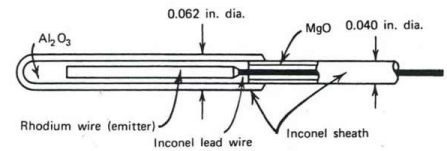
\includegraphics[width=0.5\textwidth]{img/SPD_1.png}
    \caption{Samo-napájecí detektory.}
    \label{fig:SPDKonstrukce}
\end{figure}

\subsubsection{Termoluminiscenční detektory}

Termoluminiscenční detektory jsou zařízení, která využívají schopnost některých materiálů uchovávat energii ionizujícího záření v podobě excitovaných elektronů. Když je materiál zahřátý, elektrony se uvolní z energetických pastí a při návratu na nižší energetickou hladinu vyzařují světlo.

Proces fungování termoluminiscenčních detektorů zahrnuje tyto kroky:

\begin{itemize}
    \item Ionizující záření excituje elektrony z valenčního do vodivostního pásu. Tyto elektrony jsou zachyceny v záchytných centrech.
    \item Zahřátím materiálu získají elektrony dostatečnou energii k uvolnění ze záchytných center.
    \item Při návratu do základního stavu emitují elektrony světlo, které je detekováno pomocí fotonásobiče.
\end{itemize}

Vyzařovaná energie je úměrná energii pohlceného ionizujícího záření, což umožňuje přesné měření dávky záření. 

Pro výrobu TLD se používají materiály jako lithium fluorid (LiF), calcium fluoride (CaF$_2$), magnesium beryllium oxide (MgBeO$_4$), a calcium sulfate dopovaný dysprosiem (CaSO$_4$(Dy)). Každý z těchto materiálů má různé citlivosti a energetické charakteristiky pro různé druhy záření.

Výhody termoluminiscenčních detektorů zahrnují:

\begin{itemize}
    \item Vysokou citlivost a přesnost měření.
    \item Širokou oblast lineární závislosti mezi dávkou a odezvou.
    \item Opakované použití díky možnosti vymazání zachycené energie zahřátím.
    \item Možnost použití materiálů s vlastnostmi podobnými lidské tkáni, což je výhodné pro lékařskou dozimetrie.
\end{itemize}

Nevýhody zahrnují citlivost na světlo a znečištění, což může ovlivnit přesnost měření. Termoluminiscenční detektory nejsou běžně používány v I\&C systémech jaderných reaktorů, ale nacházejí uplatnění v oblasti osobní dozimetrie.

\subsubsection{Aktivační detektory}

Aktivační detektory představují pasivní detektory ionizujícího záření, které se primárně používají k měření fluence neutronového záření. Tyto detektory mají obvykle tvar fólie nebo drátu a jsou vyrobeny buď z jednoho prvku, nebo z definované slitiny. Nejprve jsou detektory ozařovány v měřeném poli záření, během čehož dochází k indukci radionuklidů. Po ozáření se pomocí spektrometrie gama záření stanoví aktivity příslušných radionuklidů, což umožňuje výpočet celkové fluence neutronů.

Jednou z hlavních výhod aktivačních detektorů je, že jejich odezva není ovlivněna gama zářením, které je obvykle přítomné v poli neutronů. Dalšími přednostmi jsou malé rozměry a odolnost, což umožňuje jejich použití v aktivních zónách jaderných reaktorů. Pro detekci tepelných neutronů se často využívají materiály jako kobalt (Co), zlato (Au) a železo (Fe), zatímco pro rychlé neutrony se používají nikl (Ni), titan (Ti) a niob (Nb).

Specifickým příkladem použití je Aeroball Measurement System (AMS), který se používá v elektrárnách KWU. Tento systém využívá kuličky o průměru 1,7 mm vyrobené z oceli obsahující 1,5 \% vanadu. Kuličky se pohybují pneumatickým systémem (dusík) a slouží k týdenní kalibraci ostatních neutronových detektorů.

\begin{figure}[H] 
    \centering
    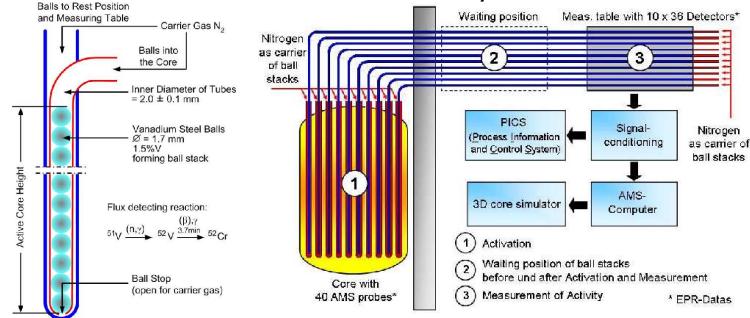
\includegraphics[width=0.5\textwidth]{img/AktivačníDetektory.png}
    \caption{Aktivační detektory v reaktoru.}
    \label{fig:AktivačníDetektory}
\end{figure}

\subsection{Charakteristiky detektorů}

\textbf{Citlivost} \textendash{} Schopnost produkovat měřitelný signál pro daný typ částic a energii. Závisí na:
\begin{itemize}
    \item účinném průřezu ionizujících interakcí,
    \item hmotnosti detektoru,
    \item šumu detektoru,
    \item tloušťce detektoru.
\end{itemize}

\textbf{Odezva} \textendash{} Vztah mezi energií částice a výstupem na detektoru (celkovým nábojem nebo amplitudou proudového pulsu).

\textbf{Funkce odezvy} \textendash{} Spektrum monoenergetického svazku je detektorem pozorováno jako komplikovaná funkce, většinou blízká Gaussově funkci s chvostem k nižším energiím.

\textbf{Mrtvá doba} \textendash{} Doba potřebná pro vytvoření a zpracování signálu v detektoru. Velmi vysoká mrtvá doba vede k navrstvení pulzů přes sebe, což následně způsobuje spektrální posun a horší rozlišení.

\textbf{Detekční účinnost} \textendash{} Poměr mezi počtem částic vyzářených zdrojem a detekovaných detektorem (absolutní účinnost). Ta se skládá z:
\begin{itemize}
    \item vnitřní účinnosti,
    \item geometrické účinnosti (akceptance).
\end{itemize}

\textbf{Energetické rozlišení} \textendash{} Nejmenší rozlišitelný rozdíl energie $\Delta E$ mezi dvěma blízkými energiemi. U monoenergetického svazku je ideálně $\delta$-funkce, reálně pík s konečnou šířkou (většinou Gaussův tvar). Rozlišení se udává ve formě pološířky (FWHM) jako relativní rozlišení $\Delta E / E$ v \%.

\textbf{Časové rozlišení} \textendash{} Nejmenší rozlišitelný rozdíl časů, definice podobná jako u energie.

\textbf{Dráhové rozlišení} \textendash{} Nejmenší rozlišitelný rozdíl v dráze, definice obdobná jako u předchozích veličin.

\subsubsection{Parametry detektorů neutronů}

\textbf{Citlivost k neutronům} \textendash{} Závisí na:
\begin{itemize}
    \item účinném průřezu konverzního materiálu a energii neutronů,
    \item objemu a hustotě detektoru (absorpce náboje).
\end{itemize}

\textbf{Energie reakce} \textendash{} Energie uvolněná záchytem neutronu ($Q$-energie), která determinuje kinetickou energii detekovatelné částice.

\textbf{Potlačení $\gamma$ záření} \textendash{} "Průhlednost" detektoru pro $\gamma$ záření v porovnání s velikostí $Q$:
\begin{itemize}
    \item větší $Q$ zajišťuje lepší odstup od šumu a $\gamma$ záření,
    \item "průhlednost" detektoru pro $\gamma$ závisí na hustotě a $Z$ detektoru.
\end{itemize}

\textbf{Možnost získání informace o energii původního neutronu} \textendash{} Kolekce celého vzniklého náboje zajišťuje spolehlivou diskriminaci a umožňuje spektroskopii. Používají se například:
\begin{itemize}
    \item konverze (n, $\alpha$),
    \item metoda odražených protonů.
\end{itemize}

\begin{table}[h!]
\centering
\caption{Parametry a jejich význam v kontextu detekce neutronů.}
\label{tab:parameters}
\resizebox{\columnwidth}{!}{
\begin{tabular}{cc}
\toprule
\textbf{Parameter}               & \textbf{Význam}                                                                                   \\ \midrule
$\Phi$ (fluence)                 & Tok neutronů (počet neutronů na jednotku plochy)                                                  \\ 
$\sigma$ (cross-section)         & Účinný průřez (pravděpodobnost interakce neutronů s látkou)                                        \\ 
$R$ (reaction rate)              & Rychlost reakcí (počet reakcí za sekundu)                                                         \\ 
$E$ (energy)                     & Energie neutronů                                                                                  \\ 
$dE/dx$ (stopping power)         & Ztráta energie na jednotku délky při průchodu částic prostředím                                   \\ 
$L$ (mean free path)             & Střední volná dráha (průměrná vzdálenost mezi interakcemi neutronů s látkou)                      \\ 
$\epsilon$ (detector efficiency) & Detekční účinnost (podíl registrovaných interakcí vůči celkovému počtu interakcí)                  \\ 
$\Delta E$ (energy resolution)   & Energetické rozlišení (schopnost detektoru rozlišit různé energie částic)                         \\ 
$T$ (time resolution)            & Časové rozlišení (schopnost detektoru rozlišit události v čase)                                   \\ 
$S/N$ (signal-to-noise ratio)    & Poměr signálu k šumu (kvalita měřeného signálu vůči šumu pozadí)                                  \\ \bottomrule
\end{tabular}
}
\end{table}

\subsection{Provozní režimy a konfigurace provozních parametrů}

\subsubsection*{Impulsní režim komory}

V impulzním režimu komory se detekují jednotlivé impulzy z neutronové komory. Signál je následně zesílen a diskriminován. Diskriminace slouží k tomu, aby byla zvýrazněna odezva na neutrony, která je nejsilnější, a naopak potlačeny impulzy s menší amplitudou, jako jsou impulzy způsobené gama, beta, alfa zářením nebo šumem. Tyto složky jsou eliminovány diskriminací. V tomto režimu je však třeba řešit problematiku mrtvé doby. Maximální četnost impulzů bývá typicky do 10$^5$ impulzů za sekundu, přičemž na zařízení VR-1 dosahuje přibližně $5 \cdot10^4$ impulzů za sekundu. Při vysokých četnostech impulzů může nastat problém stejnosměrného posunu signálu za kondenzátorem, což lze kompenzovat pomocí speciálních systémů, například systému dataPartner pro reaktor LVR-15.


\subsubsection*{Proudový režim komory}
V proudovém režimu komory se měří celkový stejnosměrný proud (DC) protékající komorou. Tento režim umožňuje potlačit mrtvou dobu, což je výhodné zejména při měření velkých hustot neutronového toku. Na druhé straně zde není možné využít standardní diskriminaci k potlačení vlivu alfa a gama záření či šumu. Proudový režim se používá pro velké rozsahy proudů, kde je vhodné využít logaritmické zesilovače nebo Campbellovu metodu, která vychází ze vztahu $n=\text{RMS}^2$. Pro potlačení vlivu gama záření se využívají kompenzované komory nebo Campbellovský režim.

\textbf{Kompenzovaná komora:}

Kompenzovaná komora se skládá ze dvou částí. První část měří jak neutrony, tak gama záření, zatímco druhá část měří pouze gama záření. Pro získání čistého signálu neutronů se odečítají proudy z obou částí podle vztahu $I_n=I_{\gamma+n}-I_{\gamma}$. Tento přístup umožňuje eliminovat vliv gama záření a získat přesné údaje o neutronovém toku

\begin{figure}[H] 
    \centering
    \includegraphics[width=0.5\textwidth]{img/KompenzovanáKomora.png}
    \caption{Kompenzovaná komora.}
    \label{fig:KompenzovanáKomora}
\end{figure}


\textbf{Campbellovský režim:}

Proudový režim, který využívá jen střídavou
složku (AC) proudu.

Campbellova metoda přináší několik významných výhod, které ji činí atraktivní pro aplikace v detekci záření. Především využití střídavých (AC) zesilovačů, které se snáze konstruují a nabízejí lepší stabilitu a menší drift ve srovnání se stejnosměrnými (DC) zesilovači.

Další výhodou je kvadratická závislost výkonu na RMS (Root Mean Square), která umožňuje pokrýt celý výkonový rozsah typicky pouze jedním měřicím kanálem.

Navíc Campbellova metoda poskytuje velmi dobrou diskriminaci gama záření, která je srovnatelná s diskriminací dosažitelnou pomocí kompenzovaných komor.

\textcolor{red}{CHYBÍ KONFIGURACE PROVOZNÍCH PARAMETRŮ!!!} 


